%%%%%%%%%%%%%%%%%%%%%%%%%%%%%%%%%%%%%%%%%
% Short Sectioned Assignment
% LaTeX Template
% Version 1.0 (5/5/12)
%
% This template has been downloaded from:
% http://www.LaTeXTemplates.com
%
% Original author:
% Frits Wenneker (http://www.howtotex.com)
%
% License:
% CC BY-NC-SA 3.0 (http://creativecommons.org/licenses/by-nc-sa/3.0/)
%
%%%%%%%%%%%%%%%%%%%%%%%%%%%%%%%%%%%%%%%%%

%----------------------------------------------------------------------------------------
%	PACKAGES AND OTHER DOCUMENT CONFIGURATIONS
%----------------------------------------------------------------------------------------

\documentclass[paper=a4, fontsize=11pt]{scrartcl} % A4 paper and 11pt font size

\usepackage[T1]{fontenc} % Use 8-bit encoding that has 256 glyphs
\usepackage{fourier} % Use the Adobe Utopia font for the document - comment this line to return to the LaTeX default
\usepackage[english]{babel} % English language/hyphenation
\usepackage{amsmath,amsfonts,amsthm} % Math packages

\usepackage{lipsum} % Used for inserting dummy 'Lorem ipsum' text into the template

\usepackage{sectsty} % Allows customizing section commands
\allsectionsfont{\centering \normalfont\scshape} % Make all sections centered, the default font and small caps

\usepackage{fancyhdr} % Custom headers and footers
\pagestyle{fancyplain} % Makes all pages in the document conform to the custom headers and footers
\fancyhead{} % No page header - if you want one, create it in the same way as the footers below
\fancyfoot[L]{} % Empty left footer
\fancyfoot[C]{} % Empty center footer
\fancyfoot[R]{\thepage} % Page numbering for right footer
\renewcommand{\headrulewidth}{0pt} % Remove header underlines
\renewcommand{\footrulewidth}{0pt} % Remove footer underlines
\setlength{\headheight}{13.6pt} % Customize the height of the header

\numberwithin{equation}{section} % Number equations within sections (i.e. 1.1, 1.2, 2.1, 2.2 instead of 1, 2, 3, 4)
\numberwithin{figure}{section} % Number figures within sections (i.e. 1.1, 1.2, 2.1, 2.2 instead of 1, 2, 3, 4)
\numberwithin{table}{section} % Number tables within sections (i.e. 1.1, 1.2, 2.1, 2.2 instead of 1, 2, 3, 4)

\setlength\parindent{0pt} % Removes all indentation from paragraphs - comment this line for an assignment with lots of text

%----------------------------------------------------------------------------------------
%	TITLE SECTION
%----------------------------------------------------------------------------------------

\newcommand{\horrule}[1]{\rule{\linewidth}{#1}} % Create horizontal rule command with 1 argument of height
\usepackage[utf8]{inputenc}
\usepackage{graphicx}
\title{	
\normalfont \normalsize 
\textsc{Hochschule f\"ur Angewandte Wissenschaften Hamburg, Department Informatik} \\ [25pt] % Your university, school and/or department name(s)
\horrule{0.5pt} \\[0.4cm] % Thin top horizontal rule
\huge Effizienzvergleich drei verschiedener Implementationen des abstrakten Datentyps SET \\ % The assignment title
\horrule{2pt} \\[0.5cm] % Thick bottom horizontal rule
}

\author{Stefan Subotin, Paul Mathia, Dennis Sentler & Philip Scheer} % Your name

\date{\normalsize\today} % Today's date or a custom date

\begin{document}

\maketitle % Print the title
%----------------------------------------------------------------------------------------
%	PROBLEM 1
%----------------------------------------------------------------------------------------
\section{Vorwort}
Getestet wurden drei Implementationen des abstrakten Datentyps Set. Im folgenden betrachten wir die Implementationen ArrayList, DoubleLinkedSet und HeapList, die über eine Schnittstelle Set, auf Effizienz sowie Vor- und Nachteile getestet wurden. Durch Verifikations- und Quantitative Tests werden diese drei Implementationen gegeneinander verglichen und auf Effizienz analysiert.\\


\section{Dokumentation der Tests}
In diesem Abschnitt beschäftigen wir uns mit den Verifikationstests die bekräftigen sollen, das die Spezifikation aller drei Implementationen erfüllt ist. 

\subsection{testeSize}
Der erste zu testende Teil war die Implementation der size() Methode. Die size() Methode liefert den aktuellen Zähler über die bereits enthaltenen Elemente.
Im Test wurde also überprüft, ob das Hinzufügen sowie entfernen von Datenelementen den eigentlich beabsichtigten Effekt auf den Element-Zähler 'size' hatte. 
Getestet wurde das Hinzufügen von 10 Elementen in ein anfänglich mit 10 initialisiertes Array. Die Menge wurde anschließend mit 1000 Elementen befüllt
und es konnten keine Laufzeitspezifischen Fehler beobachtet werden. 

\subsection{testeAddAndFind}
Im folgenden werden die Methoden add() und find() auf Erfüllung der Spezifikation getestet. Die Methode add() fügt der Menge ein neues Element hinzu und liefert nach
Erfolgreicher Speicherung das POS-Objekt mit entsprechendem Index des hinzugefügten Elements. Die find() Methode erwartet als Parameter ein Objekt vom Typ Key, der die
Eigenschaft besitzt Elemente in der Menge eindeutig anhand ihres Schlüssels(KEY) zu identifizieren. Getestet wurde erst einmal ob Elemente die der Menge tatsächlich hinzugefügt
wurden, auch gefunden werden. In sämtlichen positiven Tests wurde die korrekte POS der hinzugefügten Element zurückgeliefert. Bei den negativ Tests wurde mit Hilfe eines
Stopelements überprüft ob das gesuchte Element auch tatsächlich nicht Teil der Menge ist.  

\subsection{testeAddAndDeletePos}
In diesem Teilabschnitt wurden weitere Tests auf die bereits eingeführte Methode add() in Kombination mit deletePos() durchgeführt.Die Methode deletePos() verlangt als
Parameter ein Pos-Objekt und entfernt das Element an dem vom Dienstleister übergebenen POS Parameter. Getestet wurden sowohl valide Positionen als auch Positionen die gar
nicht im Bereich der Listen Kapazität lagen. 

\subsection{testeAddAndDeleteKey}
Hier erfolgten weitere Tests zum Entfernen von Elementen diesmal allerdings mit der Methode deleteKey, welche als Parameter ein zu einem Element eindeutigen Schlüssel erwartet,
und falls vorhanden dieses entfernt. Getestet wurden auch hier valide sowie invalide Positionen getestet und es konnten keine Fehler über JUnit Tests beobachtet werden. 

\subsection{testeAddAndRetrieve}
Die Methode retrieve() liefert - angenommen die im Parameter übergebene Pos ist gültig - das Element an der jeweiligen Pos. Die Methode retrieve() arbeitet in Ihren Grundzügen 
ähnlich wie die anfänglich beschriebene Methode find(). Auch in diesem Test auf Spezifikation wurden alle zuvor hinzugefügten Elemente wiedergefunden. Der Negativfall lief genauso unproblematisch und 
ohne spezielle oder unerwartete Vorkommnisse ab. 

\subsection{testeUnify}
Die Vereinigungsmenge einer (nicht notwendigerweise nichtleeren) Menge U von Mengen ist die Menge der Objekte, die in mindestens einem Element von U enthalten sind.
Die mathematische Richtigkeit wurde in unserem Fall eingehalten, sodass zwei Mengen die über die unify() Methode vereinigt wurden nach ihrer Vereinigung keine Duplikate enthielten und die size()Methode 
den richtigen Wert der neu erzeugten Menge lieferte.
\newpage
\twocolumn
\section{Auswertung Quantitative Tests}
\subsection{Vorgehensweise}
Um eine Aussage über die Effizienz der Implementation machen zu können werden zwei Lösch-Operationen mit einander verglichen. Da diese unterschiedlich umgesetzt sind, werden dementsprechend auch unterschiedliche Ergebnisse erwartet.\\

Umgesetzt wurde wird dies mit einem Counter. Ein Objekt dieser Klasse zählt, speichert und gibt das Resultat aus. Das Inkrementieren des Counters wird nach jedem Rechenschritt vollzogen. Dabei wurde besonders auf 'for'- und 'while'-Schleifen geachtet, da diese bei größer werdenden Sets eine ausschlaggebende Rolle spielen. Die Größe des Sets wird für die Untersuchung immer weiter exponentiell erhöht. Folgende Setgrößen werden dabei verwendet: 10^{k} : k = \left\lbrace 1, ..., 5\right\rbrace .\\

\subsection{DeleteKey}
\begin{figure}[h]
	\begin{center}
		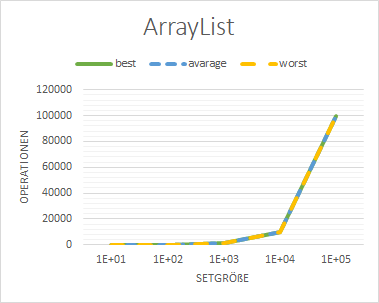
\includegraphics[width=7cm]{grafiken/DeleteKey-ArrayList.png}
		\caption{'DeleteKey' bei ArrayList verschiedener Größe}
	\end{center}
\end{figure}
\newpage
An Abbildung 3.1 erkennt man, dass die Anzahl der nötigen Operationen exponentiell mit dem Wachstum des Sets ansteigt. So groß, wie das Set ist, genau so viele Operationen müssen auch gemacht werden plus Sieben Basisoperationen die immer gemacht werden.\\ 
Was man ebenfalls erkennt ist, dass die Zugriffsrechenleistung keine Abweichungen nimmt, wenn vorne, hinten, oder in der Mitte der Liste in Element gelöscht wird.  

\begin{figure}[h]
	\begin{center}
		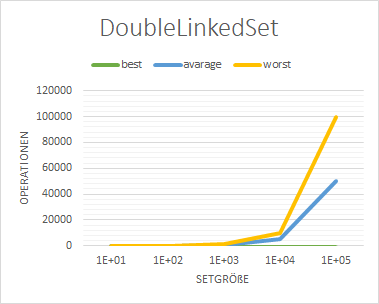
\includegraphics[width=7cm]{grafiken/DeleteKey-DoubleLinkedSet.png}
		\caption{'DeleteKey' bei DoubleLinkedSet verschiedener Größe}
	\end{center}
\end{figure}
Das DoubleLinkedSet, in der Abbildung 3.2, verhält sich allerdings anders, im Gegensatz zur ArrayList existieren optimale und weniger optimale Zugriffspunkte auf das Array des DoubleLinkedSet. Der schlimmste Fall verhält sich genauso wie die Implementation der ArrayList. Der optimale Zugriffspunkt befindet sich an letzter Position, wo die Anzahl der Zugriffsoperationen, unabhängig von der Setgröße, konstant bei Vier bleibt.
\newpage

\begin{figure}[h]
	\begin{center}
		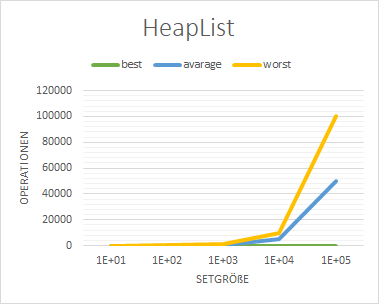
\includegraphics[width=7cm]{grafiken/DeleteKey-HeapList.png}
		\caption{'DeleteKey' bei HeapList verschiedener Größe}
	\end{center}
\end{figure}
Die Analyse des Verhaltens der HeapList aus der Abbildung 3.3 zeigt ein ähnliches Verhalten wie beim zuvor angesprochenen\\
DoubleLinkedSet. Mit dem Unterschied, dass es sich, implementationsabhängig, beim ersten Element in der Liste um das zugriffsleichte Element handelt. 

\subsection{DeletePos}
\begin{figure}[h]
	\begin{center}
		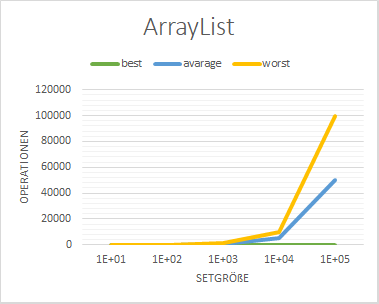
\includegraphics[width=7cm]{grafiken/DeletePos-ArrayList.png}
		\caption{'DeletePos' bei ArrayList verschiedener Größe}
	\end{center}
\end{figure}
\newpage
Implementationsbedingt bietet DeletePos aus Abb.3.4, gegenüber der getesteten Methode DeleteKey aus 3.1 einen gewissen Vorteil, denn wenn am hinteren Ende des Arrays gelöscht wird, muss nur der Array-Index um die gewisse Anzahl dekrementiert werden. Dieses Vorgehen erfordert keine Suche des Objektes, da die das Objekt durch die Positionsübergabe direkt erreichbar ist.

\begin{figure}[h]
	\begin{center}
		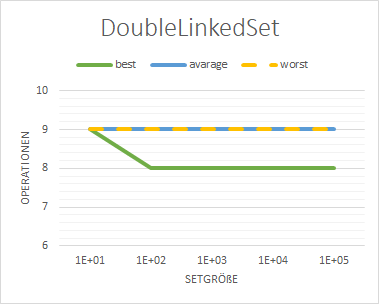
\includegraphics[width=7cm]{grafiken/DeletePos-DoubleLinkedSet.png}
		\caption{'DeletePos' bei DoubleLinkedSet verschiedener Größe}
	\end{center}
\end{figure}
Beim Löschen eines Elementes aus dem DoubleLinkedSet mithilfe eines Positionsobjektes wird, wie man in Abb. 3.5 sehen kann, kein Mehraufwand durch die Größe des Sets produziert. Da keine Suche nach dem Element betrieben wird, kann es durch das Umlinken der Indexwerte der benachbarten Elemente sehr effektiv gelöscht werden.
\newpage
\begin{figure}[h]
	\begin{center}
		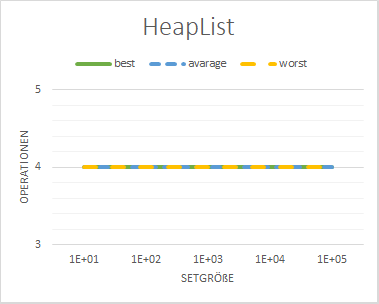
\includegraphics[width=7cm]{grafiken/DeletePos-HeapList.png}
		\caption{'DeletePos' bei HeapList verschiedener Größe}
	\end{center}
\end{figure}
Ähnlich wie bei bei dem DoubleLinkedSet der Abb. 3.5 ist bei der HeapList ein genauso effektives Entfernen der Elemente möglich, die wachsende Größe des Sets nimmt keinen Einfluss auf das Entfernen mithilfe des Positionsobjektes.  
\onecolumn
\end{document}